% !TeX root = RJwrapper.tex
\title{Image Analysis with R: a Review}
\author{Stefan R\"{o}diger, Hinrich Winther and Micha\l{} Burdukiewicz}

\maketitle

%An abstract of less than 150 words.
\abstract{
Management, display, and processing of biological and medical imaging data is 
an important task in life sciences and medical research. R is a powerful 
cross-platform statistical computing environment. The aim of this mini-review is to give a brief overview 
about image processing software for the R statistical computing environment. 
When it comes to image analysis, R may appear to provide only few tools on the 
first sight. However, a systematic analysis of the existing packages shows 
shows that a huge potential for numerous applications.
}

\section{Introduction}

\begin{itemize}
\item Digital image processing?
\item Where is it used? dffd
\end{itemize}

Scientists are using vast amount of images for qualitative data analysis. They 
originate from from technologies (e.g., fluorescence microscopy, microarrays) 
used for screening of multiple specimens of time or z-series data. For example, 
fluorescence microscopy data can be used to quantify the localization, 
localization and structure of a cell components dependent on time. Analysis of 
2D and 3D digital images is a bridge technology which has been used to unravel 
quantitative and qualitative gene expression data (mRNA and protein level), 
cellular interactions and diagnostic data. In particular, immunoflourescence 
images were analyzed in relation to cell structures, tissues and organs 
\citep{chieco_image_2013, rodiger_highly_2013, schierack_species-specific_2014, 
willitzki_new_2012}. Other applications include fluorescence-lifetime 
measurements of cellular interactions (e.g., cell adhesion), Raman-imaging and more
\citep{eliceiri_biological_2012, schierack_species-specific_2014, vogler_separation_2010}. Computational 
digital image analysis (CDIA) is a complex processcan which can yield objective 
and quantitative measurements. It involves (1) instrument control, (2) data 
import and export, (3) data connectors, (4) data storage, (5) algorithms for 
image processing and analysis, (6) machine-learning, (7) statistical analysis 
and (8) report generation \citep{eliceiri_biological_2012}. There are numerous 
software tools that have been made available for digital image acquisition and 
processing. It was shown that CDIA subtle differences within image specimens of 
multiple cellular phenotypes or cell cycle phases \citep{chieco_image_2013, 
eliceiri_biological_2012, ljosa_introduction_2009, wiesmann_review_2015}. The 
scientific background of the users is deliberately broad. This includes 
biologists, biostatisticians, physicians and others, who fundamentally make use 
of the similar image analysis techniques. From discussion with peers we learned 
that knowledge of image processing is gained by self-study. In particular, 
learning of several programming languages may hamper the scientist to focus on 
their scientific aim.

R \citep{R} is \textit{de facto} the \textit{lingua franca} of statistical 
bioinformatics and therefore used in numerous research disciplines 
\citep{rodiger_r_2015}. It is a powerful tool for statistical data analysis. It 
comes to no surprise that software packages for digital image processing have 
been implemented \citep{frery_introduction_2013}. There are numerous software 
packages for the analysis of image data \citep{wiesmann_review_2015}. However, R 
is quite functional when it comes to digital image analysis. In this review, we 
give an overview of the R ecosystem about which software packages exist and 
which deficits they may expose in comparison to other software packages. We 
aimed to aggregate information about R packages available on CRAN, Bioconductor 
\citep{gentleman_bioconductor:_2004}, RForge or github. We performed two image 
processing case studies were we applied selected packages for (A) 
immunoflourescence image analysis and (B) RMI data. 

Pixels and voxels are point samples an a grid pattern.


Multimodality imaging techniques such as CT and MRI or functional images from SPECT and PET \cite{marti-bonmati_multimodality_2010}.

Bayesian Computation in CUDA on brain fMRI data \citep{da_silva_cudabayesreg_2010}.


R version later than 2.11.0 have a graphics engine for rendering raster images via the functions rasterImage() and grid.raster() for better  scaling  of  raster  images,  faster
rendering to screen,  and smaller graphics files \cite{murrell_raster_2011}.

\section{Give me a title}

General image processing and analysis \citep{ljosa_introduction_2009}

An 3D spatial distribution analysis of biomarkers such as 53BP1, phosphorylated 
ATM, and $\gamma$H2AX  is important for an image-based modeling of dynamic 
dedistribution of DNA damage into nuclear sub-domains 
\citep{costes_image-based_2007}. The biomolecules (proteins, RNA, DNA) distribution patterns within are complex. 
Patterns range from diffuse to punctate or microspeckled 
\citep{shiels_quantitative_2007, willitzki_new_2012}. However, they all work in a coordinated and controlled 
manner within the nuleus \citep{shiels_quantitative_2007}

image processing capabilities of Cell-ID and data analysis by the statistical 
programming framework R for quantifying various cellular features (e.g., volume, 
total and subcellular fluorescence localization) from sets of microscope 
images of individual cells \citep{bush_using_2012}

\citep{tabelow_modeling_2012, tabelow_dti:_2014}

Murrel \citep{murrell_raster_2011}
\CRANpkg{mmand} \citep{clayden_mmand:_2016}

CRAN provides well established packages. These are \CRANpkg{jpeg}, \CRANpkg{png} 
and \CRANpkg{tiff} to read, write and display bitmap JPEG, PNG and TIFF images. 
The development of the \CRANpkg{ripa} \citep{frery_introduction_2013, perciano_ripa:_2014} package was 
started in 2005 by Talita Perciano. This package can be used to processes and 
analyses RGB, LAN (multispectral) and AVIRIS (hyperspectral) images. Recent 
advances of \CRANpkg{ripa} make it a promising tool for analysis of large 
datasets. The vast amount of image data is becoming more and more and essential 
part of Big Data analysis pipelines. R is among the frequently used for data 
mining and analysis. It comes to no surprise the commercial and non-commercial 
entities make heavy use of R \citep{chen_big_2014}. \BIOpkg{EBImage} 
\citep{pau_ebimager_2010} is presumably the most comprehensive package and the 
foundation for many other R packages in the context of microscopy-based cellular 
assays \citep{gowen_near_2015}. This package offers tools to transform (e.g, 
rotate) the images, segment object (e.g., cells) and extract quantitative 
descriptors. The early version of \BIOpkg{EBImage} used the Magick++ interface 
to the ImageMagick image processing library \citep{sklyar_image_2006}.

A recent package addition to this field of research is \CRANpkg{imager} \citep{barthelme_imager:_2016}.

\CRANpkg{fields} \citep{nychka_fields:_2016}

\section{General image processing and analysis}

This section may contain a figure such as Figure~\ref{figure:bead}.

\begin{figure}[htbp]
  \centering
  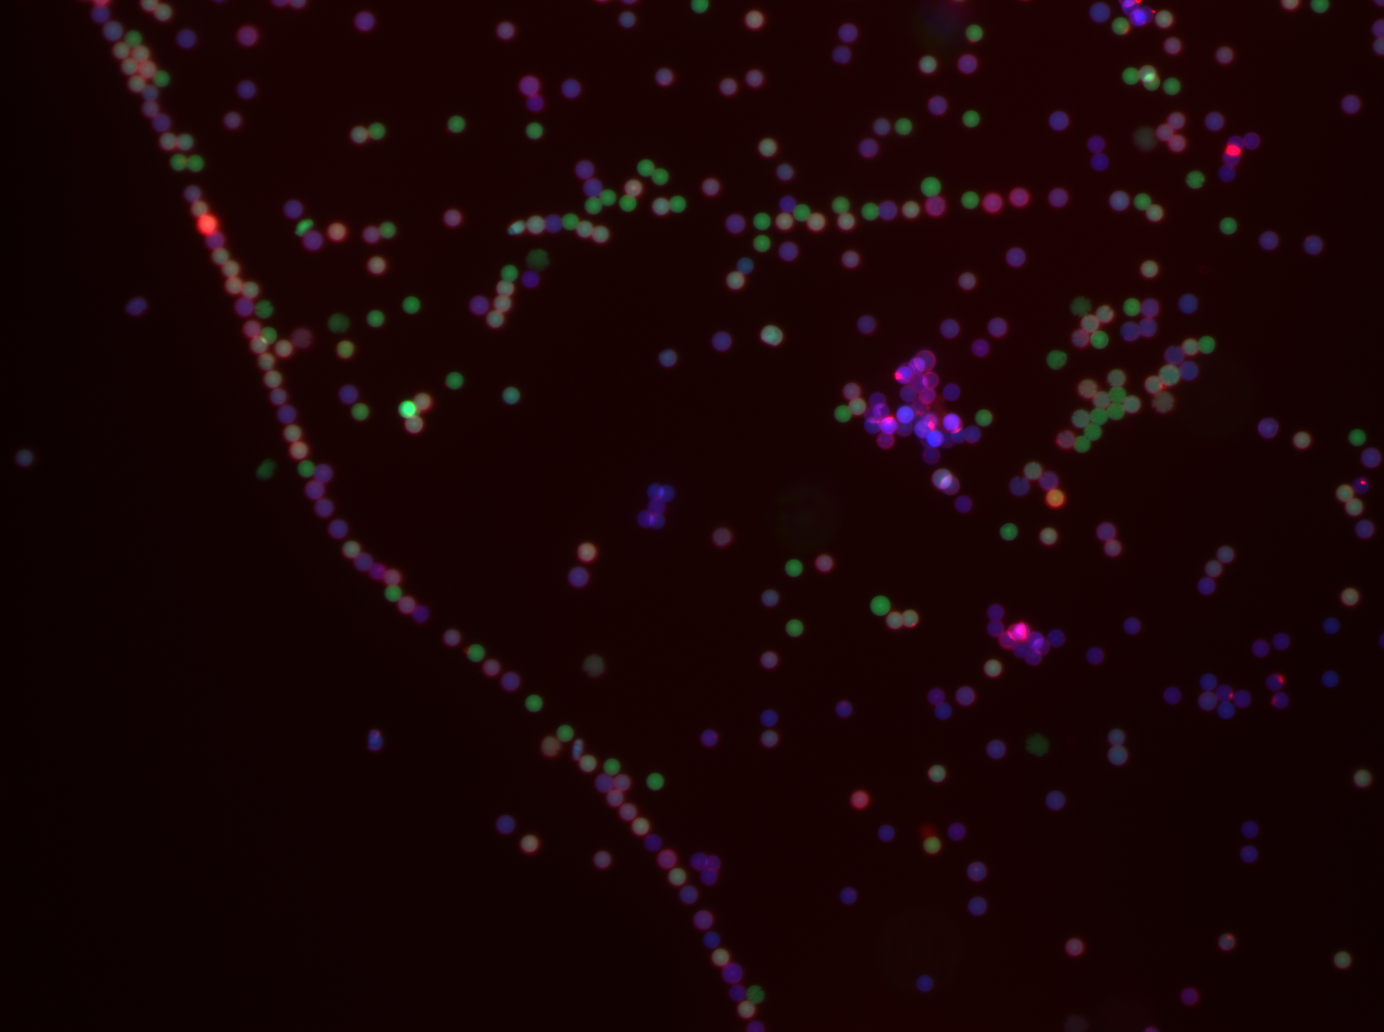
\includegraphics[clip=true,trim=0.1cm 0.3cm 0.2cm 0.1cm, width=12cm]{bead}
  \caption{Image of beads.}
  \label{figure:bead}
\end{figure}

\section{segmentation}

\citep{holmes_interactive_2009}

\CRANpkg{adimpro} is a package for manipulation of digital images and the 
Propagation Separation approach for smoothing digital images \citep{polzehl_adaptive_2007}.
For example, image analysis is used for the detection and quantification of 
cell patterns and array technologies like microarrays and bead-based assays 
\citep{dunning_beadarray:_2006, rodiger_highly_2013, willitzki_new_2012, willitzki_fully_2013}.
Several software packages have been developed. imageJ belongs to the most 
used and cited tools. When it comes to R numerous packages exist, which can 
be readily integrated in the analysis routines \citep{schultze_illuminagui_2007, frery_introduction_2013}.

The accuracy of image segmentation is a critical step in a computer-aided 
diagnosis systems. The recognition of mitotic cells and the classification of 
fluorescent patterns is heavily dependent on this. Immunofluorescent images 
of cell, such as Hep-2, exhibit a high variability due a wide range of staining 
patterns and intensity levels (FIGURES OF CELLS), the presence of mitotic 
cells and  artifacts. The later may be caused by uneven illumination and 
photo-bleaching effects \citep{tonti_automated_2015}.

Intensity inhomogeneity (bias field) is a common artefact in magnetic resonance 
(MR) images, which hinders successful automatic segmentation. \citep{ivanovska_efficient_2016}

\section{Applications}

\section{Examples}
\subsection{Statistical analysis of functional magnetic resonance imaging data}

Statistical analysis of functional magnetic resonance imaging (fMRI) data  is a 
non-invasive neuroimaging technique. R has a impressive number of packages for 
such analysis \citep{tabelow_special_2011}. They are largely used in clinical 
routine and advanced brain research. There are various R packages that can be 
used to carry out analysis compare and displaying of fMRI data \citep{muschelli-sweeney-crainiceanu:2014}.
\CRANpkg{AnalyzeFMRI} \citep{bordier_temporal_2011, marchini_analyzefmri:_2002} and \CRANpkg{fmri} 
\citep{polzehl_fmri:_2007} and are packages for the analysis of Magnetic 
Resonance Imaging (MRI) and functional Magnetic Resonance Imaging (fMRI) data, 
respectively. \CRANpkg{PET} \citep{philipsen_pet:_2010} 

 For example this 
was used to compare data from from previous studies by a meta-analysis from the 
existing literature reults \citep{stocco_coordinate-based_2014}.

Others include \CRANpkg{dcemriS4} \citep{dunning_beadarray:_2006, frery_introduction_2013}.

\subsection{Analysis of fluorescence image data}

\CRANpkg{CRImage} package \citep{failmezger_crimage:_2012} for tumor image analysis


gitter, for quantification of colony sizes from plate images \citep{wagih_gitter:_2014}


\subsection{Analysis of microbead assays}

\citep{rodiger_highly_2013, rodiger_nucleic_2014}

\begin{example}
# Detailed installation instructions are available at 
# http://bioconductor.org/packages/EBImage/

# Install the EBImage from Bioconductor
source("http://bioconductor.org/biocLite.R")
biocLite("EBImage")

# Load the EBImage package
require(EBImage)


\end{example}

\subsection{Machine Learning and Crowdsourced Data Preprocessing}
CDIA can be used to classify cells in microscopy images automatically by machine 
learning for image-based screening. \citet{sommer_machine_2013} reviewed how 
images can be converted into a data representation for machine learning (ML). ML 
functionality is present in open source packages such as CellProfiler 
\citep{conrad_micropilot:_2011, sommer_machine_2013}. CDIA R packages do not 
come with functionality. However, the R programming language has tools for 
signal processing, statistical modeling, machine learning, regression, 
classification, variable selection and data visualization 
\citep{abbas_comparative_2014, fuchs_clustering_2010, pau_ebimager_2010, 
genuer-poggi-tuleaumalot:2015}.

\texttt{example for ML and CDIA?}

Clustering is a well established and widely-used technique used in machine 
learning, data mining, character recognition and information retrieval. The aim 
is to group similar objects and separate dis-similar objects based on selected 
features \citep{szkaliczki_clustering._2016, hu_progenyclust:_2016}.  Commonly 
used algorithms, such as k-means or hierarchical clustering, require a priory 
specified cluster numbers which is often not known. Therefore clustering 
evaluation techniques were proposed. For example, Progeny Clustering can be used 
to estimate the optimal number for clustering to find the cell clusters based on 
their imaging data \citep{hu_progenyclust:_2016}.

Expert rating of images is commonly used in several stages. For example, if new 
patterens need to be classified or in cases where ambigous patterns need a 
consensus of the expert opinion. Biomedial research vast amouts of image data 
expose the scientists to a high workload. \citet{leeper_crowdsourced_2016} 
recently described the R package \CRANpkg{MTurkR} for the Amazon Mechanical Turk 
(MTurk) crowdsourcing platform, which is focused on preprocessing of data for 
immediate use in R. In his example he used crowdsourced human intelligence for 
preprocessing massive ``messy'' data into a structued form. The image rating 
task involved 225 crowdsourced workers and more than 5500 images.

Conventioanl classification algorithms operate with datasets which have a set 
of independent variables (predictor), and only one variable to be predicted. 
However, for many biomedical image data sets classifier has to work with 
several outputs. The classification of picture can have a set of labels. For 
example, pictures can be assigned landscape, sky and forest. \CRANpkg{mldr} 
package \citep{charte_working_2015} was developed for exploratory analysis, 
transformation and manipulation of multilabel datasets.

\section{Graphical User Interface for Digital Image Analysis}

There exist also R graphical user interfaces \citep{rodiger_rkward:_2012} which 
can be used for for image processing. Bio7 is an integrated development 
environment based on the Eclipse Rich Client Platform (RCP). The main purpose of 
this tool is the modeling and analysis of ecological systems. However, Bio7 is 
not restricted to this discipline. T he application contains GUIs and plugins 
for simulation and analysis tasks. Interestingly, one of these plugins is an 
adaption image application ImageJ and another is available for a bidirectional 
Java connection to R. This means that data can be transferred from and to ImageJ 
and R.

\section{Performance}

Micha\l{}, would you like to take this section?


Requirements for recent research include the rapid processing of massive amounts 
of image data (Mega to Tera byte scale) that modern technologies (e.g., 
microscopes, MRI scanner) produce nowadays. Preferably, affordable personal desktop
computers should be usable. R has several disadvantages when it comes to memory management
and GPU and CPU usage ...

\section{Orphaned R packages}

In the past there have been of R packages developed which are no longer 
maintained. 
\CRANpkg{rimage}\footnote{https://cran.r-project.org/src/contrib/Archive/rimage/ 
} provided functions for image processing, such as sobel filter, rank filters, 
fft and histogram equalization. 
\CRANpkg{edci}\footnote{https://cran.r-project.org/src/contrib/Archive/edci/} 
offered edge detection based on the difference of two asymmetric M kernel 
estimators and regression clustering (linear, circular) based on redescending M 
estimators. 
\CRANpkg{epsi}\footnote{https://cran.r-project.org/src/contrib/Archive/epsi/} 
offered edge and corner preserving smoothing methods for images which are based 
on a redescending M kernel estimator. 
\CRANpkg{biOps}\footnote{https://cran.r-project.org/src/contrib/Archive/biOps/} 
included functions for geometric, arithmetic, logic, morphologic operations, 
look-up tables, edge detection (e.g., Roberts, Sobel, Kirsch, Marr-Hildreth and 
Canny), convolution masks operations, fft, Isodata and k-means classification methods 
(standard, kd-tree, brute force methods). \CRANpkg{RImageJ}\footnote{ 
https://cran.r-project.org/src/contrib/Archive/RImageJ/} offered R bindings for 
ImageJ through \CRANpkg{rJava} to read and processes various iamge formats.

\section{Summary}

Image analysis within one software framework can help ensure that results are 
accurate, objective and reproducible. Many scientist are using R. However, it 
appears that only few make use of the image analysis tools currently available. 
We would like to raise awareness for the fact that R provides sophisticated 
packages for digital image analysis. The central advantage is that all analysis 
is conducted within the same environment across most  platforms. Added values 
for the user are that there is less need to learn a new programming languages 
and that all analysis can be performed in a consistent and cross-platform 
environment. Table~\ref{table:packages} gives an overview of R packages 
currently available. We found that functions from the packages can be easily 
combined to conduct manipulations and analysis (e.g., object transformations, 
measurements, object counting, gray level statistics, binarization) at advanced 
levels. The organization of such functions in customized packages is 
straightforward even for more complex analysis functions.

\citep{rodiger_intestinal_2015} or combined assays of microbeads and cells 
\citep{grossmann_simultaneous_2016, scholz_second_2015}

For testing purposes it is possible to make use of public image repositories as 
listed by \citet{eliceiri_biological_2012}.

Automated image acquisition systems enable microscopy experiments that generate 
large image datasets. Therefore it is important to have robust, objective and 
quantitive image analysis systems. Since most image analysis systems are 
developed for a specific type of experiment, cell type or imaging technology it 
is challenging to find one tool that fits all needs by manual adaption of all 
parameters for a specific image analysis task. Pattern recognition is a useful 
tool in this context. This can be achived by trained algorithms as described by 
\citet{shamir_pattern_2010}. 

While evaluation the packages we ended up with experiences regarding the 
installation and maintenance. Basically all installation were well instructed. 
For example, the installation of sophisticated packages like \BIOpkg{EBImage} 
is 
well documented. However, many packages depend on a number of third-party 
packages. This applies also to \CRANpkg{EBImage} which requires tiff and 
fftwtools. Similar applies to \CRANpkg{imager} which required the installation 
of fftw3 for computing Fast Fourier Transforms.

Others and we recommend to make use of packages for reproducible research 
\citep{rodiger_r_2015}. 

There exist several GUI technologies for R which make it possible to integrate 
R code into an easy to master point-and-click interface.


\begin{table}
\begin{center}
\begin{tabular}[c]{llll}
Package & Main function & Comment & Source\\
\CRANpkg{adimpro} & × & × & ×\\
\CRANpkg{AnalyzeFMRI} & × & × & ×\\
\CRANpkg{CRImage} & × & × & Bioconductor\\
\CRANpkg{dcemriS4} & × & × & CRAN\\
\CRANpkg{dpmixsim} & × & × & CRAN\\
\BIOpkg{EBImage} & fancy stuff & well maintained & Bioconductor\\
\CRANpkg{gitter} & × & based on EBImage & CRAN\\
\BIOpkg{imageHTS} & fancy stuff & - d & Bioconductor\\
\CRANpkg{imager} & × & × & CRAN\\
\CRANpkg{jpeg} & × & × & CRAN\\
\CRANpkg{PET} & × & × & CRAN\\
\CRANpkg{pixmap} & × & × & CRAN\\
\CRANpkg{png} & × & × & CRAN\\
\CRANpkg{ripa} & × & × & ×\\
\CRANpkg{RNiftyReg} & × & × & CRAN\\
\CRANpkg{tiff} & × & × & CRAN\\
\CRANpkg{rtiff} & reads and writes TIFF format images & × & CRAN\\
\emph{videoTools} & video and image analysis & - & RForge\\
\CRANpkg{webp} & reads and writes webp format images & × & CRAN\\
\end{tabular}
\end{center}
\caption{\label{table:packages}
R packages. \emph{videoTools}: http://www.rforge.net/videoTools/files/. 
\CRANpkg{pixmap} can read and write bitmap images in PBM (black/white), PGM 
(grey) and PPM (color) format.
}
\end{table}

\bibliography{roediger-winther-burdukiewicz}

\address{Stefan R\"odiger (corresponding author)\\
  orcid.org/0000-0002-1441-6512\\
  Faculty of Natural Sciences\\
  Brandenburg University of Technology Cottbus--Senftenberg\\
  Senftenberg\\
  Germany\\
}
\email{Stefan.Roediger@b-tu.de}

\address{Hinrich Winther\\
  Affiliation\\
  Address\\
  Country\\}
\email{author@work}

\address{Micha\l{} Burdukiewicz\\
  University of Wroclaw\\
  Faculty of Biotechnology\\
  Department of Genomics\\
  Wroclaw\\
  Poland}
\email{michalburdukiewicz@gmail.com}
